\documentclass[11pt]{article}
\usepackage[a4paper,left=15mm,top=10mm,bottom=10mm]{geometry}
\usepackage[OT2]{fontenc}
\pagenumbering{gobble}
\usepackage{amsfonts}
\usepackage{graphicx}
\usepackage{amsthm}
\newcommand\tsd{\theoremstyle{definition}}
\newcommand\tsr{\theoremstyle{remark}}
\newcommand\D{\displaystyle}
\setlength{\parindent}{0pt}

\tsd\newtheorem{zad}{Zadatak}
\newcommand\eng{\fontencoding{OT1}\fontfamily{\rmdefault}\selectfont}
\newcommand\srb{\fontencoding{OT2}\fontfamily{\rmdefault}\selectfont}

\title{\bf{Vezhbe iz fizike 2}}
\author{\Large Aleksa Vuchkovic1, 3c}
\date{}

\begin{document}
\maketitle
\large

\textbf{\Large Vezhba 4. Omov zakon za celo strujno kolo}\\
\textit{Odredjivanje elektromotorne sile i unutrashnjeg otpora izvora jednosmerne struje}\\

\addtolength{\tabcolsep}{5pt}
\begin{tabular}{|c@{\hspace{10pt}} *{7}{|c}}
\hline
Broj Merenja & $R [\Omega]$ & $\Delta R[\Omega]$ & $I[ 10^{-3} A ]$ & $\Delta I[ 10^{-3} A ]$ & $ I^{-1}[ A^{-1} ]$ & $\Delta I^{-1}[ A^{-1} ]$\\ [1ex]
\hline
1 & 20,0 & 0,7 & 49,8 & 0,7 & 20,1 & 0,3\\ %{0,29}\\
\hline
2 & 30,0 & 0,8 & 38,3 & 0,6 & 26,1 & 0,5\\ %{0,888}\\
\hline
3 & 40,1 & 0,9 & 29,9 & 0,5 & 33,4 & 0,6\\
\hline
4 & 50,1 & 1,0 & 24,5 & 0,5 & 40,8 & 1,0\\
\hline
5 & 60,1 & 1,1 & 20,8 & 0,4 & 48,1 & 2,0\\
\hline
6 & 70,1 & 1,2 & 18,0 & 0,4 & 55,6 & 2,0\\
\hline
7 & 80,1 & 1,3 & 15,9 & 0,4 & 62,9 & 2,0\\
\hline
8 & 90,2 & 1,4 & 14,3 & 0,4 & 69,9 & 2,0\\
\hline
9 & 100,2 & 1,5 & 12,9 & 0,4 & 77,5 & 3,0\\
\hline
\end{tabular}\\[5mm]

$\Delta R_1=1\%R_1+5d$\\
$\Delta I_1=1\%I_1+2d$\\[0.5mm]
$\Delta I_1^{-1}=\displaystyle\frac{\Delta I_1}{I_1^2}$\\[2mm]

$I^{-1} = \displaystyle\frac{1}{\epsilon}R + \displaystyle\frac{r}{\epsilon}$\\
Crtamo grafik zavisnosti $I^{-1}=f(R)$, gde je koeficijent prave jednak $\displaystyle\frac{1}{\epsilon}$, a presek sa ordinatom je $\D\frac{r}{\epsilon}$.\\[2mm]

$A = (24\Omega, 22.5 A^{-1})$\\
$B = (96\Omega, 74 A^{-1})$\\

$k=\D\frac{I^{-1}_b - I^{-1}_a}{R_b - R_a} = \D\frac{(74-22.5)A^{-1}}{(96-24)\Omega} = \D\frac{51.5}{72}\cdot\frac{1}{V} = 0.71527\D\frac{1}{V}$\\[3mm]
$\delta_k = \D\frac{\Delta I^{-1}_b + \Delta I^{-1}_a}{|I^{-1}_b - I^{-1}_a|} + \D\frac{\Delta R_b + \Delta R_a}{|R_b - R_a|} = \D\frac{3.0+0.5}{51.5} + \D\frac{1.6+0.8}{72} = 0.101294$\\[8mm]
$\Delta k =\delta_k \cdot k = 0.101294\cdot 0.71527\D\frac{1}{V} = 0.07245\D\frac{1}{V} \approx 0.08\frac{1}{V}$\\
$(k \pm \Delta k) = (0.72 \pm 0.08)\D\frac{1}{V} = \D\frac{1}{\epsilon}$\\[5mm]

$\epsilon = \D\frac{1}{k} = \D\frac{1V}{0.71527}=1.398V$\\
$\Delta\epsilon = \D\frac{\Delta k}{k^2} = \D\frac{0.07245V}{0.71527\cdot 0.71527} = 0.1416V \approx 0.2V$\\[5mm]
$(\epsilon\pm\Delta\epsilon)=(1.4\pm0.2)V$\\

\newpage
Odredili smo elektromotornu silu, sad nam preostaje josh otpor izvora, koji dobijamo iz preseka prave sa $y$-osom...\\

$n=5.5A^{-1}$\\
$\Delta n=\Delta(I^{-1})_{max}=3.0A^{-1}$\\

$r=n\cdot\epsilon = 5.5A^{-1}\cdot 1.4V=7.7\Omega$\\
$\Delta r=r\cdot(\D\frac{\Delta n}{n}+\D\frac{\Delta\epsilon}{\epsilon})=7.7\Omega\cdot 0.6883 = 5.3\Omega \approx 6\Omega$\\

$(r\pm\Delta r)=(8\pm 6)\Omega$\\

Grafik na milimetarskom papiru se mozhe videti na sledec1oj strani dokumenta.

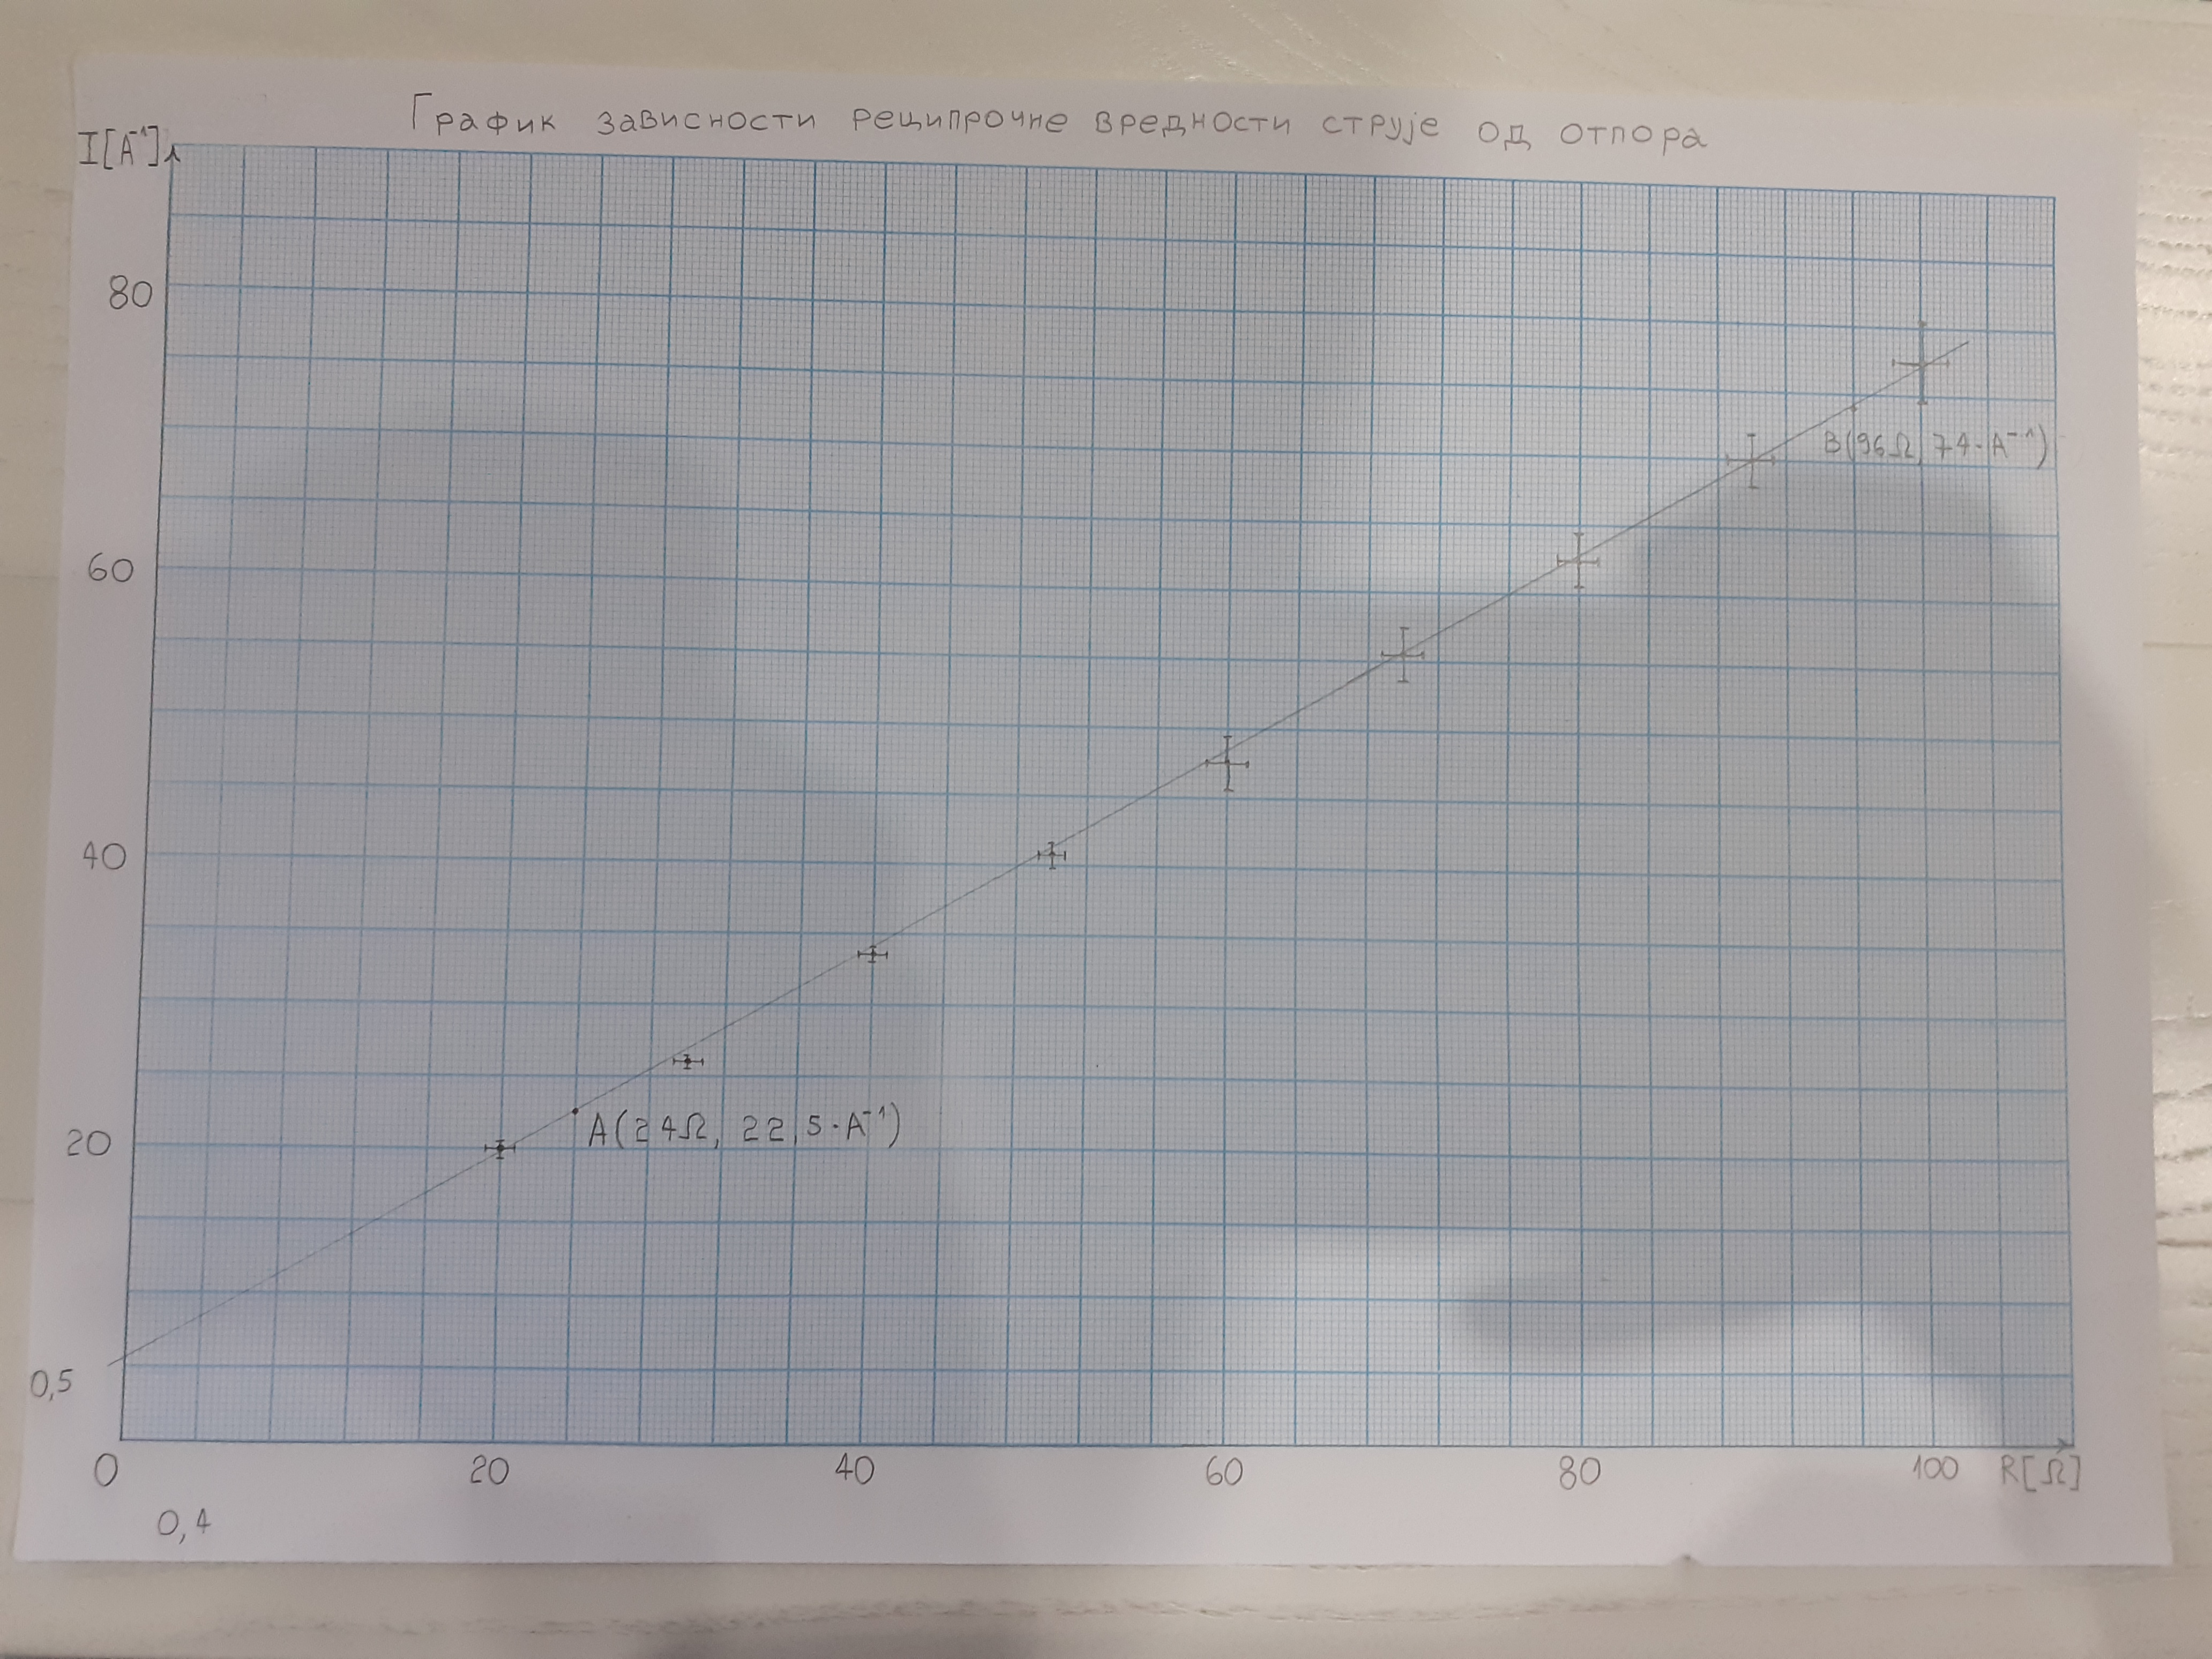
\includegraphics[angle=270,scale=0.16]{slika.jpg}
\end{document}